\documentclass[urop]{socreport}
\usepackage[pdftex]{graphicx}
\usepackage[english]{babel}
\usepackage{rotating}
\usepackage[utf8]{inputenc}
\usepackage{hyperref}
\usepackage{natbib}
\usepackage{makeidx}
\makeindex

\setlength{\oddsidemargin}{0cm}
\setlength{\evensidemargin}{0cm}
\setlength{\textwidth}{16cm}
\setlength{\textheight}{23cm}

\pagestyle{headings}

\begin{document}
%%%%%%%%%%%%%%%%%%%%%%%%%%%%%%%%%%%%%%%%   COMMANDS %%%%%%%%%%%%%%%%%%%%%%
\newcommand{\screenshot}[1]{\includegraphics[scale=0.4]{screenshots/#1.jpg}}
\newcommand{\graphic}[1]{\includegraphics[scale=0.8]{graphics/#1.jpg}}
\newcommand{\example}[1]{``{\tt #1}''}
%%%%%%%%%%%%%%%%%%%%%%%%%%%%%%%%%%%%%%%%%%%%%%%%%%%%%%%%%%%%%%%%%%%%%%%%%%

\pagenumbering{roman}
\thispagestyle{empty}

\begin{center}

\includegraphics[scale=0.1]{./graphics/EURACE-Flag.jpg} \hfill

\includegraphics[scale=0.5]{./graphics/6fp.jpg}

\end{center}
%\vspace{1cm}


%\begin{tabular}{p{4.5cm}p{12cm}}
\begin{center}
Project no.\\
035086\\
Project acronym \\
\textbf{EURACE}\\
Project title\\ 
\small{\textbf{An Agent-Based software platform for European economic policy design with heterogeneous interacting agents: new insights from a bottom up approach to economic modeling and simulation}}\\
\end{center}

%\vspace{0.1cm}

\noindent Instrument STREP \\
\small{Thematic priority IST FET PROACTIVE INITIATIVE ``SIMULATING EMERGENT PROPERTIES IN COMPLEX SYSTEMS"}\\
%\vspace{0.1cm}
\begin{center}
\textbf{Deliverable reference and title} \\
\small{\textbf{D8.2: Development of inference tools and of a friendly user interface}} \\
Due date of deliverable: \\
28/02/2009 \\ 
Actual submission date: \\
31/05/2009
%September 3rd 2008 \\

\vspace{0.1cm}
Start date of project: September 1st 2006 \hfill
Duration: 36 months \\
\end{center}

\noindent \small{Organisation name of lead contractor for this deliverable} \\
TUBITAK-UEKAE\\

\hfill Revision 1 \\

\vspace{0.3cm}
%\begin{comment}
\begin{tabular}{|l|l|c|}
\hline
\multicolumn{3}{|l|}{\small{Project co-funded by the European Commission within the Sixth Framework Programme (2002-2006)}}\\
\hline
\multicolumn{3}{|l|}{Dissemination Level:}\\
\hline
PU & \small{Public} &\\
\hline
PP &\small{Restricted to other programme participants (including the Commission Services)}&   \\
\hline RE & \small{Restricted to a group specified by the consortium (including the Commission Services)}&   \\
\hline CO & \small{Confidential, only for members of the consortium (including the Commission Services)}& X \\
\hline
\end{tabular}
%\end{comment}
%\pagebreak

%\vspace{0.5cm}
%\textbf{Attachments:}\\
%\begin{tabular}{p{1cm}p{14cm}}
%1&Software on CD \\
%2 & Software User Manual\\
%\end{tabular}
%\pagebreak


\tableofcontents
\listoffigures
%\listoftables


\chapter{Executive Summary}
Creation of software utilities for use in design of agents, design of agent populations, preparation of simulations, and visualization of simulation results has been an essential objective of EURACE project in order to present a complete platform to facilitate use of agent based simulations in policy design. The EURACE Graphical User Interface (GUI) presented here refers to a collection of compatible software tools which provide the components that correspond to these functions of the EURACE software platform.

Design of the EURACE GUI reflects our intention that these software tools reflect most general definition of the particular problems they intend to solve in agent based approach, to the extend that it is possible, while at the same time they are complete in the sense that they can be deployed in the EURACE project. In particular that they work with the FLAME simulation framework \citep{HOLCOMBE:2006}.

Following are the components of EURACE GUI that correspond to different aspects of simulation development work:
\begin{description}
\item[XMML Editor] Agent design requires a tedious process of describing agent memory and behavior in an XML format specific to FLAME (the so called XMML format) while controlling for consistency of design in terms of parameters that affect the overall model. The XMML Editor provides a graphical interface which allows the agent designer to focus in his/her job, in addition to providing facilities for detecting errors in the design. It was named after the fact that it translates the design into the XMML format which is usable in FLAME framework.
\item[GXparser] Once a model composed of several agent types is designed, it has to be compiled by the so called XParser component of the FLAME. The GXparser provides a graphical tool to ease this manual process and report possible compilation errors back to the designer.
\item[PopGUI] A population corresponding to the European Economy in EURACE simulations is composed of multiple (thousands) copies of several types of agents in several geographical regions, whose memory and relations with each other are characterized by statistical features derived from actual data. The PopGUI component enables simulation designers to describe composition of populations and statistical features of agents, and produce population instances that are used as initial states for simulations.
\item[ExpGUI] Policy experiments require comparison of outcomes of alternative simulations, where the compared cases correspond to covariation of several parameters among their corresponding ranges. ExpGUI facilitates creation of a series of simulation tasks from description of the experiment, thus reducing errors in creation of policy experiments.
\item[VisGUI] The VisGUI component provides a tool for visualization and analysis of simulation outcomes.
\item[ConGUI] Since simulation development requires several iterations over the various tasks described above, the ConGUI component was added to the EURACE GUI to ease launching of the various components described above.
\end{description}

\begin{figure}[h]
  % Requires \usepackage{graphicx}
  \centering
\screenshot{congui}
  \caption{EURACE GUI}
  \label{figure:congui}
\end{figure}
Figure~\ref{figure:congui} is the flow diagram and the graphical user interface of the toolkits developed for EURACE. The deliverable presented here first describes the architecture of EURACE GUI in relation to other components of the EURACE Software Platform, then proceeds to instructions for using various components of the GUI as part of simulation development work.




\chapter{Introduction}
This document serves as the definitive documentation for the suite of user level programs that are created as part of the EURACE project effort. The EURACE project aims to produce socio-economic models and multi-agent simulation software for use in economic policy experiments. The project has started in September 2006, and will conclude in September 2009. Information on EURACE project can be found at \url{http://www.eurace.org}.

An important requirement for EURACE project was creation of a software platform for design and implementation of agents, creation of agent populations, creation and execution of experiment sets, and evaluation and visualization of simulation results. While an existing multi-agent framework (FLAME/Xagents framework) was adopted in EURACE project and improved as part of the project effort \citep{Greenough2007}, such tools for pipeline of agent, population, and experiment design not existed at the time and created as part of the EURACE project. 

The set of user interface tools in EURACE software platform, collectively called here as EURACE-GUI, were distributed individually during early stages of project. This documentation provides a single entry introduction to capabilities and usage of EURACE-GUI. Up-to-date information about the EURACE-GUI can be accessed online at \url{http://eurace.cs.bilgi.edu.tr}.

EURACE-GUI consists of several independent modules that were created at different stages of the project. Various different technologies were employed for each module in order to satisfy implementation and agile development needs. For this reason modules are written using different computer languages (C++, Python), and uses various software and libraries (GTK, Qt, R-project). Despite their independence, the modules in EURACE-GUI can be invoked easily from within an entry point program called Control GUI (ConGUI).

These independent modules all correspond to stages of the process of designing, running, and evaluation multi-agent simulations of complex systems. Following is a brief description of each module in the EURACE-GUI:
\begin{description}
\item[ConGUI]: ConGUI is a front-end which facilitates invocation of different modules of EURACE-GUI easily as part of a design pipeline.
\item[XMML-Editor]: Used for designing different types of agents, their memory variables and behavior, in addition to global constants and messages used in a multi-agent system.
\item[GXparser]: Used as a front-end for validating agent models produced with XMML-Editor, by parsing them through FLAME's xparser.
\item[PopGUI]: Used for creating populations of agents whose state variables and relations can be initialized according to given criteria.
\item[ExpGUI]: Used for creating sets of experiments using agent models and populations, then for executing them on a FLAME simulation engine.
\item[VisGUI]: Used for visualization and statistical analysis of simulation outcomes.
\end{description}

The reader is recommended to read Chapter \ref{ch:overview} which provides an overview of the multi-agent model, population and experiment design process, before proceeding to subsequent chapters which explain usage of individual modules. 

 
\chapter{Requirements and Installation}
EURACE-GUI is written with portability in mind. Despite the variety of libraries it depends upon, all such dependencies are available for common computing platforms including 32-bit or 64-bit variants of GNU/Linux, Unix or BSD, and Microsoft Windows. While it is likely that it can be run on other systems such as Mac OS, it is neither tested on those platforms not we provide installation packages for them. Manual installation of individual modules of EURACE-GUI and libraries required by them can be cumbersome. Nevertheless, details of doing so are described in Appendix \ref{ch:manualinstall} and module sources can be downloaded from \url{http://eurace.cs.bilgi.edu.tr}.

Before installing EURACE-GUI using installation packages, you are recommended to install the following software separately:
\begin{description}
\item[FLAME]: FLAME multi-agent platform is developed and distributed by University of Sheffield. Please check \url{http://ccpforge.cse.rl.ac.uk} for FLAME installers.
\item[R]: R statistics package installers are available for a variety of platforms and is distributed under the GPL license. R installers can be downloaded from \url{http://www.r-project.org}.
\end{description}
Although you can install and run EURACE-GUI without having the above software, you should be aware that created simulations cannot be run without FLAME platform, and most features of the VisGUI component will not be available without R. However, if your intention is merely using a computer as a multi-agent design workstation, it is perfectly possible to install and run EURACE-GUI without these two software packages.

\section{Installing required software}
Although EURACE-GUI can be installed and run without the following software, its use and features are limited without them. Therefore it is recommended that the following are installed, in this order:
\begin{description}
\item[R]: R statistics package can be downloaded and installed from \url{http://www.R-project.org}. If you are using a Debian or Ubuntu Linux, it can also be installed using the package `r-base'.
\item[FLAME]: First get the sources from \url{http://ccpforge.cse.rl.ac.uk}. After unzipping the sources, you need to compile and install two components from FLAME tree: libmboard and xparser. Enter to these directories in the given order, run `make' then `make install'.
\end{description}

\section{Installing EURACE-GUI from binary distribution}
To get a copy of EURACE-GUI installer, go to \url{http://eurace.cs.bilgi.edu.tr} and download the most recent binary package for your platform (supported platforms are Windows, Linux and other Unix variants). Execute this file to complete the installation.

\section{Installing EURACE-GUI from sources}
If you are working on Microsoft Windows, MinGW is required to compile and install the EURACE GUI from sourse distribution. It can be downloaded from \url{http://www.mingw.org}. On Ubuntu or Debian Linux platforms you will need to have the package named build-essentals installed. Once you have this built environment for your platform, follow the instructions in Appendix \ref{ch:manualinstall}.

\chapter{Overview of Agent and Population Design Process}
\label{ch:overview}
Certain stages of multi-agent simulation design envisioned in EURACE depend on output of other stages. Figure \ref{fig:workflow} visualizes the flow of work through modules in EURACE-GUI, also indicating the type of data that comes out from modules and used as input to others. This visualization is exactly what you will see when you launch the ConGUI, which acts as  the control panel for invocation of different modules in EURACE-GUI.
\begin{figure}
\caption{Flow of multi-agent design in EURACE}
\label{fig:workflow}
\graphic{workflow}
\end{figure}

The first stage in EURACE multi-agent simulation design is creation of agents and shared environment using XMML-Editor. Agent design involves (1) designing agent memory for different types of agents, (2) describing agent behavior, in the case of EURACE/FLAME the language used for such description is C programming language using a few FLAME specific constructs, (3) designing global environment variables shared by agents, (4) designing data types that occur in memory variables and exchanged as data units between communicating agents. Use of XMML-Editor to carry out these tasks is described in Chapter \ref{ch:xmme}. Once the multi-agent model design is completed, the model is saved in a FLAME specific format called XMML. 

The next stage is designing a population of agents which will be the initial state of simulation. The model created in XMML-Editor is used as an input to PopGUI, which enables one to specify how different geographical regions in the simulated system are composed of different number of each type of agents, how each agent's memory should be initialized, and what should be the values of environment constants shared by all agents. PopGUI provides a variety of expressions which can be used to specify random distributions for initializing agent memory, or to establish relations between agents (e.g. employment relations in an economic simulation). Using these specifications PopGUI can create population instances which are different but has the same stochastic properties.

The model and a population instance is sufficient to run a simulation. The model contains what are the memory variables of agents and program code describing their behavior. The population instance on the other hand contains initial values of agent memory for a whole set of agents comprising the population. Before a simulation is run however, the model must be compiled to generate an executable. The GXparser module allows user to do this without going down the elaborate steps of xparser program in FLAME. 

Economic simulations are useful when one can compare outcomes of different environments, populations, or behavior. The ExpGUI program provides facilities to create a set of different initial conditions (populations) and to run simulations easily.

Finally the VisGUI program can be used to visualize and analyze the results of simulations. The program use plotting and statistical facilities of R statistics package \citep{Rproject}.
\chapter{Agent Design with XMML-Editor}
\label{ch:xmme}
XMME (X-Machines Modelling Editor) provides the functionality of
designing and implementing agent specification and behavior. It is a
GUI application and the XMML (X-Machines Markup Language) provides the
underlying modeling schema.

In particular, XMME helps its user to visually edit an XMML formatted
file. XMML is a highly verbose and partially untyped data
specification language based on XML format. This sort of nature makes
it relatively difficult to edit individual XML files to describe
agents' specification and behavior which are very sophisticated in so
far that the agents have internal variable and external message
dependencies. Furthermore, the nested model fascility of XMML
specification makes it virtually unmanageable if it comes to large
models.

The XMME wraps the XMML specification and functionality by means of
nested data models. In its runtime, all the decoupled XMML files and
XMML nodes are managed by the application so that the model
specification remains consistent over time. By doing this, XMME does
not limit the XMML capabilities which allow to represent sophisticated
agent models, on the contrary, it helps modeler to deal with the
technical details and internal model specification consistency.

\bigskip

XMME is a free and open source software application which is developed
using C++ and Trolltech/QT development framework. The development idea
is based on content-presentation seperation, ie. the model internals
are controlled by a seperate routine which is a software library
called \texttt{libxmm2}. \texttt{libxmm2} provides the model whereas
XMME presents it to the user. At the same time, it passes all the user
input to the \texttt{libxmm2}. \texttt{libxmm2} is written purely in
C++ and core QT library which means that it can be used by any other
software routine, such as web server applications, command line
programs etc. During the EURACE software toolkit development phase,
developers have made extensive use of this library with
fast-prototyping principles. Beyond \texttt{libxmm2}, XMME uses QT's
model-view classes, which makes it easy to align to XMML while new
functionalities added to XMML specification.

Both XMME and and \texttt{libxmm2} are cross-platform applications. So
far, it has been ported to Microsoft Windows, GNU/Linux and MacOSX
operating systems.

\bigskip

XMME GUI design is based on two panes. Left pane provides a
hierarchical tree-view widget where all the XMML nodes are
represented. The right hand pane allows the user to edit available
nodes in detail.

A screenshot is provided below on Table \ref{xmmescreen}

\begin{figure}
  \centering
  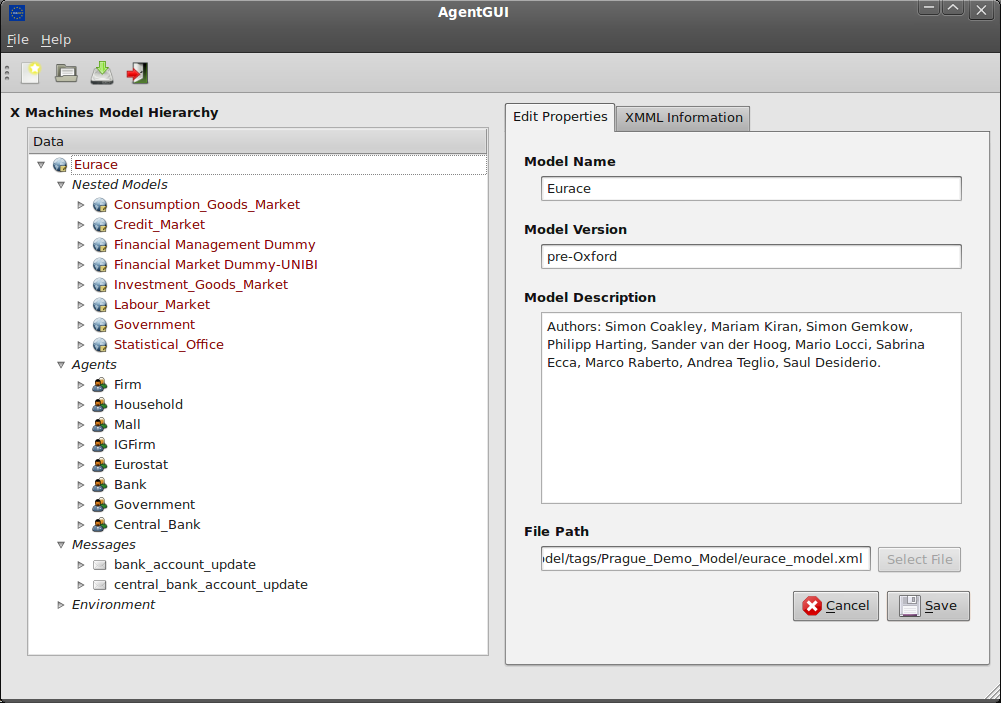
\includegraphics[width=14cm]{screenshots/xmmescreenshot.png}
  \caption{XMME (AgentGUI) Screenshot}
  \label{xmmescreen}
\end{figure}
\chapter{Compiling Agents with GXparser}
Once a model composed of several agent types and markets is designed, it has to be compiled by the so called XParser component of the FLAME.  The GXparser module of EURACE Toolkit is essentially a graphical user interface wrapper of XParser. It eases the manual process of economic design and report possible compilation errors back to the designer. See Figure~\ref{figure:gxparser}.
\begin{figure}[h]
  % Requires \usepackage{graphicx}
  \centering
\screenshot{gxparser}
  \caption{GUI for XParser}
  \label{figure:gxparser}
\end{figure}

\chapter{Population Design with PopGUI}
PopGUI is written for creating agent populations for EURACE  Project simulations using FLAME multi-agent framework. The program reads already designed agent models described in FLAME XMML format, and provides facilities to specify composition of population and specifications for initializing each agent's memory variables. Populations created by the program is then exported as an XML file (so called 0.xml file in FLAME), which can be fed into a simulation engine which uses these initial conditions and agent behavior described in models to carry out the simulations.

When reading through this guide it is important to distinguish the terms `population' and `population instance'. PopGUI's central concern is to maintain specifications for creating initial populations. `Population' refers to these specifications and the program stores them in its own format in '.pop' files. Many `population instance's(0.xml files) can be created from the same population specification. Although PopGUI is designed to create valid population instances, the program does not read them back or allow their manipulation.

Population specification involves two main phases. First is population composition. In the FLAME framework an agent population can be divided into any number of sub-populations. For example, the EURACE model contains geographical regions, such as countries, and one can distribute the agents among these regions using the PopGUI. One most straightforward example is countries of the world. Although each country's social life is composed of same types of agents such as workers/consumers, firms, banks, etc., their compositions and demographic features are different since each country have a different population (number of people), number and average size of firms, etc. To account for such realistic populations, PopGUI allows its user to create several regions and specify numbers of each type of agent separately for each region; therefore allowing each region to have a different composition.

The second phase of specifying a population involves assigning values to agents' memory variables. Each type of agent is described by a different set of variables. For example employees can be described with their skill set, income and employment status, whereas a firm is described by number of workers, production capacity, etc. For a realistic population one usually needs standard or empirical random  distributions. For instance in our economic world example, sizes of firms in a country usually shows a normal distribution, although its mean is different for each country/region. PopGUI provides a rich set of expressions to specify memory variables.

Another feature of a realistic population is that the agents in it are not isolated but relate to one another. For example workers are employed by firms in their region, or firms borrow money from banks in their country. Therefore these relations must also be initialized in order to create a population, and they must be stored in agent memory variables. In the case of employment relation example, firms will have employees whose skillset is suitable for what firm produces, and furthermore the relation is exclusive (i.e. if a person is employed in a firm, he/she cannot be employed by another). In the firm-bank relation example firms usually borrow money from banks in their own region, and the relation is not exclusive (i.e. other firms also borrow money from the same bank). PopGUI provides a rich set of features for creating relations between agents, both exclusive and otherwise. 

In additional to those substantial features mentioned above, some rather practical features were also implemented to address needs of agent modelers. For example agent models change through time. New agent types may be added, or agent memory variables are changed. It would be quite impractical to start over with the population design when such changes occur. For this reason PopGUI allows importing population specifications from populations that were worked out for older versions of models. With the help of this feature populations can be re-used with only incremental changes. Such features are introduced in the relevant sections below.

\section{Using PopGUI}
In order to create populations with PopGUI, you need a model describing your agents (their memory and behavior). Since PopGUI was written as a part of EURACE project, it currently can use only  models given in XMML format, which is the format of the FLAME framework, the official simulation environment of EURACE. Similarly the population instances created by the program are exported only in the XML format adhering to FLAME specifications. 

Although agent models contain behavior in addition to memory of agents, only the agent memory is of interest when creating populations. Agent behavior is used later by the simulation engine, along with the population created by PopGUI.

Working out a population with PopGUI consists of several stages:
\begin{enumerate}
\item Create a population by choosing a model, choosing the number of regions in simulation, and optionally importing previous work from an existing population.
\item Specify population composition by entering how many agents of each type will exist in each region.
\item Specify how agent memory variables will be initialized. This also means specification of relations between agents since relations are expressed as an agent's identification number appearing as a value in some other agent's memory.
\item Enter values of global environment constants.
\item Create one or more instances of population.
\end{enumerate}
Each of stages are described in the sections below.

\section{STEP 1: Creating a population}
First create a new population, from file menu. When creating a population you'll be asked for the model xml file which must be in FLAME XMML format. Then you can give a name to the population and set the number of regions in the window that pops up, as shown in Figure \ref{fig:properties}. The default number o regions is 1. You can increase this number depending on your needs. When you are finished you must save your changes using ``Update and close'' button in the properties dialog. You can later view or change these properties using the ``Properties'' button in the toolbar. The update operation only updates the population in your session, and does not save the changes in the file system. To save your changes permanently at any point, you must use ``Save population'' or ``Save population as'' menu items from the ``File'' menu group. The population information is saved in a file with `.pop' extension in your file system.
\begin{figure}
\screenshot{properties}
\caption{Population properties dialog}
\label{fig:properties}
\end{figure}
If you want to use a previously created population, click the ``Open population'' menu in the ``File'' menu group, then choose a population. Alternatively the name of a `.pop' file can be given as a command line argument to PopGUI when invoking the program (see section \ref{sec:cmdline} about command line options below).

Once you have a population loaded to PopGUI, pressing ``Model summary'' button will display a rudimentary structure of the model you have chosen, for inspection purposes. 

Note that there's also an ``import...'' button on the properties dialog. The import feature is provided for a practical concern in modeling work. Once a population is created, PopGUI forgets about the original model and only remembers agents and their memory variables. However the agent models may change while work on population continues. It would be quite impractical to start over entering population specifications every time the model changes, and when the changes are minor (e.g. a few memory variables are added or updated in the model). In such cases what you need to do is to create a new population using the newest model, and then import your previous work into the new population using this ``import...'' button on the properties menu. However special care must be paid since import operation will import agent memory variable specifications for only those that exists in your latest model. Therefore if there are newly added memory variables or agents, it is up to you to complete the specifications for such new variables and agents.

A restriction of import operation is that number of regions in the current population must match that of the population you are importing from. Therefore even if you plan to change number of regions, you must do so only after importing.

NOTE: As new features are added to PoPGUI it may not stay backwards compatible. For ensuring stability data structures used by PopGUI are given a version number. If you try to open an old population with newer versions of the PopGUI there is a chance that it will fail with a warning about the versions. The recommended way to handle such situations is to create a population from scratch and import memory variables as described above.

\section{STEP 2: Specifying population composition}
Next step is to set number of each type of agent in each region. When you click ``Edit Regions'' button in the toolbar, you will be presented a table whose columns are regions and whose rows are agents (see Figure \ref{fig:regions}). You can enter the number of agents in this grid and then press ``update and close'' button if you want to save these changes. Your entries must be either positive integers or zero. 
\begin{figure}
\screenshot{regions}
\caption{Editing population composition}
\label{fig:regions}
\end{figure}

\section{STEP 3: Specifying agent memory variables}
This is the most elaborate step of specifying populations in PopGUI. When you press ``Edit memory variables'' toolbar button, you will be presented with a detailed display of agents and their variables with several buttons at the bottom part of screen, as shown in Figure \ref{fig:memvars}. Agents, their memory variables, and sub-components of these memory variables are presented in the form of a tree, parts of which can be collapsed or expanded by clicking on the branches. Alternatively all branches can be expanded or collapsed using the ``Expand all''/''Collapse All'' buttons at the bottom of the screen. 
\begin{figure}
\screenshot{memvars}
\caption{Editing memory variables}
\label{fig:memvars}
\end{figure}

This display also have a grid structure since one must provide specification for memory variables separately for each of the regions. However in most cases the specifications for different regions of the same variable are same or very similar. For this reason a ``Region copy'' button is provided in this screen. Using this feature you can copy specifications for one region to other regions, and then make incremental changes, to speed up your work.

As described above, specifications of memory variables are elaborate and has two basis: values and relations. Although both are addressed in the language used for memory variable initialization (or 'initform' as we refer to them in EURACE), different features are required and thus we will present them in separate sections below. The 'syntax help' button on the memory variables screen displays up-to-date reference on the initform language for your convenience. As a note to users, the initform language is based on dynamic interpretation capability of Python, and hence it has a Pythonic syntax. However. it is not necessary at all for users to have any experience in Python language (although a little bit can help if one wants to use lambda expressions for extending the initform language as will be shown below).

\subsection{Distinguishing simple and composite variables}
Next to each variable's name in the memory variable editing screen, you will see a variable type. Following are the varieties of these types:
\begin{itemize}
  \item A few variables are special. Currently these are the ones named `id' and `region\_id'. Users cannot enter anything for these variables. The `id' is a unique identifier of each agent in the population (for referencing purposes) and it will be assigned sequentially during population instantiation. This variable must exist for FLAME simulations to work. `region\_id', when used, will contain an integer which is the number of the region in which the agent is placed.
  \item Some variables are STATIC or CONSTANT. These appear in cases where their value is fixed in the model or taken from a constant. The names of constants are defined in agent model, but their values are entered in PopGUI using ``Edit constants'' toolbar button.
  \item Simple variables has a type which is one of `int' or `double'.
  \item Composite variables are actually C structs. The names and structure of these come from agent model which is used when creating a new population. When a variable is of a composite type, its sub-fields can be expanded and will be entered in separate boxes.
  \item Finally, a variable can be an array of a simple of composite type. For such variables users will enter a specification for the length of array in addition to the variable (which is used for each element of the array). Special features are provided when one wishes to address all elements of an array, such as when they will be selected from a set without replacement.

Most common use of STATIC or CONSTANT variables occur in array sizes, in cases when array size is fixed in the model either hard coding or by tying to a constant.
\end{itemize}

\subsection{Specification syntax for variables and basic random distributions}
The entries for memory variables are arithmetic expression which produce a single numeric value (except the special case of array initialization). Therefore the expressions entered into the boxes in this screen can be as simple as a constant number, or a simple arithmetic expression: e.g. \example{2} or \example{2*2-(3.14/4)}. Whenever necessary, PopGUI will convert integer values to real numbers, or vice verse.

In most cases the values will not be constants. Use of random or deterministic initializations are very common. Following functions are provided for use in such cases in initforms:
\begin{description}  
   \item[rand(int,int)]: a random integer from the inclusive range.
   \item[rand(real,real)]: a random real number from the range.
   \item[choice([v1,v2,...])]: Pick a value from the list randomly.
   \item[normal(mu, sigma)]: Normal distribution. mu is the mean, and sigma is the standard deviation. 
   \item[discrete( (probability,value), (probability,value),... )]: Choose value given discrete probabilities. Probabilities must add up to 1.0.
\end{description}

Also you can combine any of the above in arithmetic expressions: e.g. \example{2+rand(0,5)} or \example{rand(2,6)+choice([1,3,6])}, etc. Discrete versions of random distributions are automatically chosen by PopGUI. In other words even if you use \example{random(1.0,2.0)} for a variable whose type is integer, it will be automatically treated as  \example{random(1,2)} by PopGUI.

The expressions you enter are essentially Python expressions which must produce a single value (with the exception of array initialization, see Section \ref{sec:arrayinit}). If you have some knowledge of Python, you can enter any valid expression combining the special functions provided by PopGUI. 

While entering specifications, the ``Syntax help'' button on the bottom of this screen can provide you a quick reference help, as an alternative to this user manual. Once you are finished entering specifications you can use the ``Validate'' button on this screen to ensure that your expressions are correct. This validation is mostly a syntactic one and does not guarantee that you will be able to generate a population instance at the end. That depends on various things including setting up of relations, and its success cannot be determined before you actually proceed to create an instance.

\subsection{Deterministic initialization}
\example{deterministic(min,max, lambda function)} will assign values by taking one value at a time from inclusive range and applying function to selected value. Min and Max must be integer, and Max must be greater than Min. e.g. \example{deterministic(0,10,lambda x:x*10)} will initialize the memory variable of a sequence of agents as:
     \begin{verbatim}
      agent[0]=0
      agent[1]=10
      ...
      agent[10]=100
      agent[11]=0
      ...
     \end{verbatim}
\subsection{Using other memory variables of agent in expressions}
It is possible to use value of a memory variable of agent itself in specification of another. The \example{getSelfVar()} function is provided for this purpose. For example if agent has two memory variables of simple types named `numberofchildren' and `monthlyexpenses', one can depend on the other by entering \example{getSelfVar("numberofchildren")*1250+2000} in the box for `monthlyexpenses'. 

However you must be careful about dependencies of variables. PopGUI will analyse which other memory variables a variable depends on and sets their values in proper order. But if there are cyclic dependencies which cannot be satisfied, you will face an error at some point.

In the example above \example{getSelfVar()} returned simply a numeric value since the named variable was a simple variable. However, if the memory variable referred to is an array or a composite type, rather than a simple variable, one usually needs to further refer to its elements. For example if the returned value is an array \example{getSelfVar("somearray")[0]} will return first (zero indexed) element of it. If the returned value is a composite variable \example{getSelfVar("somecomposite")["x"]} will return its sub-field named `x', and so on.

The \example{getSelfVar()} cannot be used to refer to the variable itself, for example to access sibling variables in a data structure, etc. For this purpose another function is provided: \example{getSibling("sibling var name")}. When used in an array of data structure, this function will retreive the data field of the current array element. In cases where a data structure contains other data structures or elements, getSibling() can instead access higher levels in the data structure hierarchy using 'level' parameter to climb up the hierarchy. For example \example{getSibling("uncle X",level=1)} and \example{getSibling("grand uncle Y",level=2)} will seek entities at the level of parent and grandparent in the data structure hierarchy, respectively.

\subsection{Initializing arrays}
\label{sec:arrayinit}
The only case where the result of your expression is allowed not to be a single numeric value is when you want elements of an array specified at once. In this case your expressions must yield a list whose length is the same with the array length. For example if you have an array of length four, you can use something like \example{[1,2,3,4]} to initialize the array elements sequentially from this list. A few functions whose return values are lists are provided for possible use in such cases:
\begin{description}  
   \item[sample([1,2,3,...],k)] : Return a k length list of unique elements chosen from the sequence. Used for random sampling without replacement.
   \item[permutation([x,y,z,...])]: Return the same list with elements randomly re-ordered.
   \item[sequence(start,end,increment), realsequence(start,end,increment)] : generate a sequence of integers with given increment within the inclusive interval: [start, start+increment, start+2*increment, ..., END] where END$\le$end. rsequence is the version which works for real numbers
\end{description}

\subsection{Using model constants or population size for scalability purposes}
You can access model constants or number of agents in the population using the following:
\begin{description}
   \item[getConstant(constantname)]: Returns the value of model constant. e.g. \example{getConstant("alpha")} to retrieve the value of constant named "alpha". (These constant values are what you set in the ``Edit constants'' tab of the program).
   \item[getAgentCountGlobal(agentname)]: Get global count of agents with given name, i.e. sum of number of agents in all regions. e.g. \example{getAgentCount("Firm")}
   \item[getNumRegions()]: Returns the number of regions in the population.
   \item[getAgentCountRegional(agentname)]: Get regional count of agents with given name.
   \item[getAgentIDListRegional(agentname, agentname, ...)]: Get a list of agent IDs. You may specify name of one or more agents. Please note that agent names are case sensitive. i.e. if you named an agent as ``Firm'' you must specify the exact name. The function is deterministic, ie. when called several times the list of agent IDs will be in the same order.
   \item[getAgentIDListGlobal(agentname, agentname, ...)]: Get a list of agent IDs. You may specify name of one or more agents. Please note that agent names are case sensitive. i.e. if you named an agent as ``Firm'' you must specify the exact name.  The function is deterministic, ie. when called several times the list of agent IDs will be in the same order.
\end{description}
Since the last two functions return a list, rather than a value, they are usually intended for array initialization.

\subsection{Accessing other agents and initializing agent relations}
Agents are not isolated. For example employees and firms in an economics simulation are related to one another through employment relations. To address this aspect of populations PopGUI provides a means to select other agents in the population using some criteria, and use their memory variables in specifying another agent's memory.

In order to pick an agent one can use:
\begin{description}
%\item[getAgentByID(agentname,ID)]
\item[getAgentRegional(agentname, conditions=[("varname",condition), (..), ...])]
\item[getAgentGlobal(agentname, conditions=[...])]
\end{description}
%The first function returns the agent with given ID. 
The first one selects an agent from the same region with the referring agent, and the second selects one from the whole population. The selectios are random. Both functions can be provided with zero or more conditions on the agent to be selected using the following format:\\
\example{getAgentRegional("Bank", conditions = [ ("givescredit",equals(1)), ("badreputation",equals(0), ... ] ) }\\
Please note that conditions is a list of tuples {\tt (variable name, condition function)}. Variable name must be a variable of the selected agent, and condition is one of the special functions defined. These functions can be one of the following:
\begin{description}
   \item[equals(what)]: checks whether the value of selected variable equals  to the value
   \item[between(a,b)]: checks whether the value of selected variable within the range
   \item[contains(x)] is the value of selected variable (which must be a list) contains the value
   \item[MooreNeighbour(numcolumns,no)]: checks whether the variable (an integer) is in the Moore neighbourhood of "no" in a geography where regions are laid out in rows with a width of 'numcomulmns'. For example if there are 9 regions laid out as follows:
      1    2    3
      4    5    6
      7    8    9
    then neighbours of region 1 are 2,5,4, whereas neighbours of region 5 are1,2,3,4,6,7,8,9, etc.
   \item[your own functions]: Other conditions can be defined using so called lambda functions in Python language, such as  \example{lambda x: x<100 and x>=5}. For example \example{getAgentRegional("Employee", conditions = [ ("skill",lambda skill : skill<100 and skill>50) ] ) }
   \item[subequals(index,what)]: checks whether x[index]==what
   \item[subsubequals(index1,index2,what)]: checks whether x[index1][index2]==what
\end{description}

Once an agent is selected, its variables can be accessed using a function called \example{getAgentVar(variablename)}. For example: \example{getAgentGlobal("Bank", conditions = [ ("region\_id", MooreNeighbour(10,getSelfVar("region\_id") ) ] ).getAgentVar("id")}. If the selected variable is a struct or a list, its elements can be accessed using a syntax similar to the examples given for \example{getSelfVar()}, e.g. \example{getAgent("Bank").getAgentVar("interestrates")["shortterm"]}.

The agents are selected randomly by the current implementation of the above functions in PopGUI to prevent procedural bias in selection.

\paragraph{Exclusive selection}
If one wishes to prevent others from selecting the same agent, it is possible to do so by setting the 'exclusive' flag to 1 in getAgent variants, i.e. \example{getAgentRegional("Employee",exclusive=1)}. Once you do this, the selected employee will never be selected again. However one must be careful since it is possible, depending on the composition of the population, that such conditions may not be satisfied once all agents are taken.

\paragraph{Selecting multiple agents at once}
Two similar functions allow one to select all agents that match the criteria, instead of only one:
\begin{description}
\item[{getAllAgentsRegional(agentname,conditions=[])}]
\item[{getAllAgentsGlobal(agentname,conditions=[])}]
\end{description}
The variants accept same arguments as \example{getAgentRegional()} and \example{getAgentGlobal()}. However what is returned is a list of agents. These functions has an optional argument which can be used to turn of random shuffling of the returned agent list. For example getAllAgentsRegional("Firm",randomize=0) will always return the same list in the same order.
 

If one needs to process specific variables of the agents selected, you will need Pythonic expressions as in the following example:\\
\begin{verbatim}
 sum([ agent.getAgentVar("somevar") 
   for agent in getAllAgentsRegional("Bank", 
         conditions=[("givescredit",equals(1)),("badreputation",equals(0))]) ])
\end{verbatim}
The above expression is based on a Python construct which computes a list from elements of a given list, e.g. \example{[i*i for i in [1,2,3]]}

\subsection{A note about managing dependencies}
 The group of functions getAgentGlobal/Regional() and getAllAgentsGlobalRegional() create a dependency between agents.
 In some cases this creates cyclic dependencies which cannot be resolved by the PopGUI. If desired you can
 solve such situations by using one of the two functions. First is signaling a delayed execution of memory variable initialization:
\begin{verbatim}
   delayedExecution("some expression"): the expression is executed after all agents and their variables are executed. 
\end{verbatim}
 to evoid syntax errors due to quotes in your own expressions, use long string syntax in Python by putting
 your expression in triple quotes. e.g.:
\begin{verbatim}
   delayedExecution(\"""getAgentGlobal("Bank").getAgentVar("id")\""")
\end{verbatim}
 
 Another function is available to fine tune dependencies at the level of variables instead of agents:
\begin{verbatim}
   dependencyFineTune(type,toagent,tomemvar,expression)
e.g.:
   dependencyFineTune("Global","Government","gov_id",
     \"""getAgentGlobal("Government",conditions=
     [("regions",MooreNeighbour(3,getSelfVar("region_id")))]).getAgentVar("gov_id")""")  
\end{verbatim}


\subsection{Some useful Python constructs}
Python has a simple syntax and some simple constructs can prove useful in expressing your memory variables. We present some constructs here that are observed to be of common use based on feedback from our users. For further information you are advised to consult Python tutorial at its website \url{http://www.python.org}.
\begin{description}
\item[Constructing lists]: range(start,end[,step]) constructs a list which includes start but not end. If given the list is incremented with the given step value.
\item[Lambda functions]: An anonymous function can be constructed using lambda function syntax. For example a function to return true if a number is even would be `lambda x: x%2==0'
\item[List processing]: A new list can be produced by processing numbers in a given list. For example to return squares of a range of numbers `map(lambda x:x*x, range(1, 11))'.

If what you want is to select only items from a list that match a criteria, use filter. For example to select even numbers from a list: `filter(lambda x: x%2==0, [1,2,4,5,7])' (will return [2,3]).

\end{description}
\subsection{FINISHING UP: Validating and saving memory variable specifications}
Before saving memory variables you can use the 'Validate' button on the window, which provides elementary syntax checking of expressions you enter. After validation use ``Save and close'' button on the memory variables screen to save your entries.

The validation operation only validates expression syntax and does not attempt a full initialization and checking of expressions and references for fitness. Thus you may still catch some problems when you attempt to instantiate population later.

%\subsubsection{Cautions for large populations}
%When creating large populations use of functions getAgentGlobal(), getAgentRegional(), getAllAgentsGlobal(), and getAllAgentsRegionsl() will slow down the process since they scan all agents of selected type to check whether they meet the criteria. If your intention is to use all agents of a certain type, it is recommended to use the getAgentIDListRegional/Global() first to obtain a list of agents, and then accessing individual agents using getAgentByID(). For example the first form below will take much more time than the second:
%\begin{verbatim}

%\end{verbatim}
\section{STEP 4: Editing constants}
The constants defined in your model will be assigned a value of zero initially. You can change these values using the ``Edit Constant'' toolbar button. The constants screen also have a ``Validate'' button to ensure the expressions you have entered are valid, before you save them.

Instead of numbers, you can also use getAgentCount("agent name") as a value for constants.

Unless you set sensible values to constants, it is likely that you will get errors like ``division by zero'' when you validate memory variable specifivations that use these constants.

\section{STEP 5: Instantiating population and finishing up}
Once you finish entering memory variables and update your changes using the 'save and close' button, you can create an instance of the population (i.e. the 0.xml file in EURACE parlance) using 'Instantiate population' button. You will be asked for the name of the file to export the population. 

Depending on the number of agents in your population this process can take a long time, and the progress will be displayed on the main screen. You can cancel this operation using the ``Cancel'' button at any time.

Once you are finished working with your population remember to save it before you quit the program. Later you can re-open them from the file menu, and create new population instances for the same population. Different instances will not be the same but will have same statistical distributions adhering to your specifications.

\section{Command line options, utilities, and debugging}
\label{sec:cmdline}
PopGUI accepts a few command line options when run from command line instead of from within ConGUI. Use:
\begin{verbatim}
python popgui.py -h
\end{verbatim}
to display help on these options. Option ``-v'' will display program version, and ``-d'' will turn on debugging so that program will dump a lot of messages in the terminal it is being run, which can be helpful in reporting bugs. 

Also you can give a population file as command line argument for the program to open the population during start up. For example:
\begin{verbatim}
python popgui.py -d test.pop
\end{verbatim}
will open the population saved in ``test.pop'' and will turn on debugging while you work.

PopGUI uses versioning for the saved populations to identify the data structure changes that are not backwards compatible, and denies to open populations that were created using past versions of the program and are not compatible with the current version. You can disable version checking using ``-i'' parameter at the command line, however it is strongly recommended that such usage should be avoided.

Distributed with the PopGUI is a small program named popdoc.py, which  is for producing \LaTeX tables for constants, population composition, and memory variables in the population specification. When the program is run without any parameters, it will ask a few questions to produce desired output. When given a tex file as command line argument, output is written to that file instead od screen.

\section{NOTES}
\begin{enumerate}
\item {\bf Avoiding dependencies whenever possible}: The group of functions getAgentGlobal/Regional getAllAgentsGlobal/Regional create dependency between agents. We have seen modelers using these functions just to retrieve id's of other agents. However the correct way to do that is to use getAgentIDListGlobal/Regional. This is because  all agents are created and  given id's before any of them are populated with memory variables. Therefore retrieving agent id's does not generate any dependency, and is a faster operation.
\item {\bf Resolving dependencies}: If you end up with a cyclic dependency, the first thing you can try is to use delayedExecution()
\item {\bf Be careful with Lambda functions}: When describing conditions in agent selection, you may resort to using Python Lambda functions. However you must beware that lambda functions are evaluated when they are called, not when they are created. For example if you want to choose agents whose regionid is same with the choosing agent, you'd try a function like \example{lambda x:x["regionid"]==getSelfVar("regionid")}. However the function is executed within the context of agent being evaluated for selection, because of the inherent way how Python lambda functions are evaluated. (This was the reason that functions such as subequals() subsubequals() were created.)
\item {\bf Using external replicators to create hude populations}: If you start PopGUI with `-r' option, the created xml files will have all agent ID numbers preceeded with the string `REPLACE\_ID\_'. 
\end{enumerate}
\chapter{Running Simulations through ExpGUI}
%\subsection{Integration with Experimental GUI}
\subsection{The EURACE GUIs}
\subsection{Integration}
It was thought at first that the job submission bash shell scripts could be used by the experimental GUI for remote working, even on a Windows machine using Cygwin or MSYS. A later decision to make the Windows GUIs work natively meant that this could not happen and so an alternative implementation has been necessary. By making use of paramiko (\verb+http://www.lag.net/paramiko/+) and implementation of the SSH2 protocol for python, the remote execution and copying of files has been implemented to run natively on all platforms.  Scripts that run on the remote machine have been left as bash scripts as all the compute clusters run some version of Linux or Unix and the existing remote host configuration files can be used. 

At present from the experiment GUI the user can:

\begin{itemize}
\item choose the remote host
\item specify a serial or parallel job
\item specify the number of processes for a parallel job
\item run the job
\item check on job status (if remote system uses batch processing)
\item retrieve results.
\end{itemize}

Resource constraints have meant that it has not been possible to implement the full requirements of Projects containing Jobs within the experimental GUI.


\chapter{Analysis of results using VisGUI}
\section{Overview}
The VisGUI design takes an advanced GUI workspace approach where designers or policy makers can import, visualize, analyze, edit and export simulation results.

The VisGUI architecture is designed aiming an overall modular implementation. It employs a Model View Controller(MVC) scheme, which enables its modularity and extendability. Although the package is a sub-module within EURACE Software Toolkit, it can be installed and run independently. This design decision is taken for several reasons. First, this flexibility is targeted to allow it to be integrated for other multi-agent computational tools as an analyses and visualization tool. For that reason, importation and exportation of standard data formats are adopted for better interoperability. Second, it allows designers or policy makers easily install and run VisGUI to perform analyses and visualizations of simulations data which are generated elsewhere. Third, this decoupling feature allowed us to develop the application upon existing GPL\footnote{GNU Public License, see url{http://www.gnu.org/}} licensed tools and software. In return, after a maturation stage of the application, the package will be made available publicly on public repositories\footnote{Such as url{http://sourceforge.net/}} as a GPL package. This will enable a contribution back to the open source community and contribution from the developers from the community to extend and maintain it in the future.
\begin{figure}[h]
  % Requires \usepackage{graphicx}
  \centering
\screenshot{db}
  \caption{Parallel Database Creation}
  \label{figure:db}
\end{figure}
\begin{figure}[h]
  % Requires \usepackage{graphicx}
  \centering
\screenshot{db2}
  \caption{Parallel Database Creation}
  \label{figure:db2}
\end{figure}

\section{Features}
A set of features are developed and made available to designers. The features are briefly listed below and some snapshots of their use are given accordingly to ease presentation:
\begin{figure}[h]
  % Requires \usepackage{graphicx}
  \centering
\screenshot{VisGUIScreenshot}
  \caption{Visualization of Time Series a Variable}
  \label{figure:visTS}
\end{figure}
\begin{itemize}
\item \textbf{Importing Simulation Results:} The user is made able to import either result of a single simulation or a set of it. If this option is opted, the application reads in a sample iteration and retrieves information on the set of agents and their available memory variables. This automatically detected set of memory variables are used automatically to populate variable menus.
\item \textbf{Database Creation:} The creation of a database is necessary when there is a very long and large simulation. It is also necessary when there are a set of policy experiment results. Created database speeds up time to visualize and analyze the results. It also allows portability of experiment results in a standard and light format to other platforms and visualization applications. We have taken a novel approach to integrate database creation into the application. It exploits multi-threading and parallelisation paradigms both to decrease the time of database creation and to keep doing analysis at the main workspace during any lengthy process of database creation. See Figure~\ref{figure:db} and Figure~\ref{figure:db2}.
\begin{figure}[h]
  % Requires \usepackage{graphicx}
  \centering
\screenshot{visdistro}
  \caption{Visualization of Distribution of a Variable}
  \label{figure:visdistro}
\end{figure}
\item \textbf{Visualization of Time Series of Memory Variables:} The nature of simulation necessitates a quick trace of some variables over iterations before further examination or more advanced policy experiments. User can directly check raw simulation data to examine time series of a memory variable. See Figure~\ref{figure:visTS}.

\item \textbf{Visualization of Distribution of Memory Variables:} In the same manner as a quick time series visualization of raw data, users are also allowed to examine distribution of a variable at a desired iteration.See Figure~\ref{figure:visdistro}.

\item \textbf{Advanced Visualization of Policy Experiments:} The application also allows designer to examine impact of a policy parameter on macro results, sensitivity of the computational model to an initialization and effects of random interactions in between agents across different runs by advanced visualization tool of the application. The feature allows to examine multiple variables at the same time very quickly. See Figure~\ref{figure:advancedTS}.
\begin{figure}[h]
  % Requires \usepackage{graphicx}
  \centering
\screenshot{advancedTS}
  \caption{Visualization of Advanced Time Series Plots of an Experiment}
  \label{figure:advancedTS}
\end{figure}
\item \textbf{Automatic Report Generation of Data Points:} This feature allows designers to view summary statistics and exact data points of visualization of a variable.
\item \textbf{Exporting Raw Data of Plots:} The feature allows to export data points of a plot in standard data format, presumably to be tested or re-visualized by a different application. See Figure~\ref{figure:export}.
\begin{figure}[h]
  % Requires \usepackage{graphicx}
  \centering
\screenshot{export}
  \caption{Exporting Raw Data of Plots}
  \label{figure:export}
\end{figure} 
\item \textbf{Managing Generated Reports and Plots:} Analyses and visualizations of an experiment results in many reports and plots. This set of feature allows user either visualize or close them easily or automatically store them on a secondary memory space.
\item \textbf{Automatic Storage and Re-storage of State of Application:} This feature allows both the main application and all interactive GUI dialogs to store its latest state for subsequent uses.
\item \textbf{GUI Interaction and Validity Checks:} All of GUI dialogs are interactive to user preferences and automatically checks validity of user actions.
\begin{figure}[h]
  % Requires \usepackage{graphicx}
  \centering
\screenshot{fileop}
  \caption{File Operations}
  \label{figure:fileop}
\end{figure}
\item \textbf{Writing and Editing Reports:} VisGUI Workspace provides a text editor with basic functions to enable user to write reports or edit automatically generated reports for convenience.
\item \textbf{Logging Status and Actions in the Workspace:} All major user actions are logged and displayed. The user can scroll and examine his/her previous actions.
\item \textbf{File Operations:} All basic file operations including printing options are provided. See Figure~\ref{figure:fileop}.

\item \textbf{Configuring Workspace:} The application provides configuration options for the workspace, its state, and automatic management of produced plots and reports. See Figure~\ref{figure:config}.
\begin{figure}[h]
  % Requires \usepackage{graphicx}
  \centering
\screenshot{config}
  \caption{Configuring Workspace}
  \label{figure:config}
\end{figure}
\item \textbf{Help Menu:} VisGUI provides an HTML based navigable help interface. 
\end{itemize}

\section{Using VisGUI}
In this section, we will very briefly demonstrate how VisGUI can be used. 

\subsection{Platforms}
VisGUI is developed and tested both in Linux and Windows environments. The application will also be adopted for MAC platforms.
\subsection{External Packages}
The application is being implemented using Python2.5 and Qt4. All distributional statistics, and time series analysis and inference analysis are being performed by employing and integrating RPy2. RPy has provided an efficient and practical Python interface to the R Programming Language. More specifically, the software is implemented using Python 2.5 with the help of following packages:
\begin{itemize}
\item GUI: PyQt4.QtGui
\item XML: PyQt4.QtXml
\item Statistics: RPy 2
\item DB: SqlLite
\end{itemize}

\subsection{Standalone Installation}
The modular design approach of VisGUI allows it to be installed and used as a standalone application. This flexibility will allow the package to be later developed as an platform and economic model independent workspace which can be used to analyse and and visualize results of other computational economics platforms.

\section{Summary}
The section has presented a brief overview of VisGUI. The modular approach of the its implementation and its major design principles will provide us to further develop it and share it with computational economics community in the future.


%%%%%%%%%%%%%%%%%%%%%%%%%%%%%%%%%%%%%%%%%%%%%%%%%%%%%%%%%%%   APPENDICES   %%%%%%%%%%%%%%%%%%%
\appendix
\chapter{Manual installation from sources}
\label{ch:manualinstall}
\section{Installing PopGUI}
PopGUI is written in Python language for faster development and portability reasons. It uses GTK+ for its graphical user interface, Therefore PopGUI will run on any platform for which Python (version 2.5 or higher) and GTK+(version 2.0 or higher) is available, including GNU/linux, Microsoft Windows, most Unixes, and others.

The program itself consists of two files only: poplib.py which contains the library functions, and popgui.py which provides the GUI. Follow the instructions below for your operating system to start using PopGUI.

\subsection{Installation on GNU/Linux}
Install python-gtk2 package. Then place poplib.py and popgui.py into some directory, and run popgui.py. If you want to do these from a command line, do as follows (example for Debian or Ubuntu Linux):
\begin{verbatim}
 $ sudo aptitude install python-gtk2
 $ python popgui.py
\end{verbatim}

\subsection{Installation on Windows}
Install the following in order (See \url{http://www.pygtk.org/downloads.html} for detailed instructions and links for setting up Python with GTK support):
\begin{enumerate}
\item Python 2.5 or newer
\item GTK+ win32 runtime
\item PyCairo
\item PyGObject
\item PyGTK
\end{enumerate}

After that copy poplib.py and popgui.py into a directory, and run popgui.py.

%%%%%%%%%%%%%%%%%%%%%%%%%%%%%%%%%%%%%%%%%%%%%%%%%%%    BIBLIOGRAPHY  %%%%%%%%%%%%%%%%%%%%%%
\bibliographystyle{plain}
\bibliography{eurace}
\end{document}
